\documentclass[8pt]{article}

\usepackage{clj-grammar}
\usepackage{amsmath, listings, amsthm, amssymb, proof, xspace}

%%------------------------------------------------------------------------
%% DEFINITION HELPERS
%%------------------------------------------------------------------------

%\newcommand{\alt}{~~|~~}
\newcommand{\comp}[1]{\llbracket #1 \rrbracket}

\newcommand{\inlinexp}[1]{
{\footnotesize
 \[\begin{array}{l}
 #1
 \end{array}\]}}

\newcommand{\inlinexpa}[2]{
{\footnotesize
 \[\begin{array}{#1}
 #2
 \end{array}\]}}

\newcommand{\infr} [3] [] {\infer[\textsc{#1}]{#3}{#2}}
\newcommand{\iand}        {\qquad}

\newcommand{\Ctxt}       {\mathcal{E}}
\newcommand{\InCtxt} [1] {\Ctxt[#1]}


%%------------------------------------------------------------------------
%% REDUCTION RELATION MACROS
%%------------------------------------------------------------------------

\newcommand{\subst} [3]    {#3 [#2 / #1]}
\newcommand{\dstep} [2]    {#1 ~\Downarrow~ #2}

\newcommand{\ssosredex}        {\rightarrow}
\newcommand{\ctxtreduce}       {\mapsto}
\newcommand{\sstep}     [3] [] {#2 &\ssosredex&  #3 &\textsc{#1}}
\newcommand{\ctxtstep}  [3] [] {#2 &\ctxtreduce& #3 &\textsc{#1}}


\usepackage{amsmath}
\usepackage{mdframed}
\usepackage{booktabs}
%\usepackage{enumerate}
%\usepackage{fancyvrb}
%\usepackage{amsfonts,graphicx}
%\usepackage[usenames, dvipsnames]{color}
%\usepackage{tikz}

%\setlength{\parindent}{4em}
%\setlength{\parskip}{1em}
%\renewcommand{\baselinestretch}{1.5}

\bibliographystyle{abbrv}
\include{bibliography.bib}

\usepackage{graphicx}
\graphicspath{ {images/} }

\newcommand{\tabitem}{~~\llap{\textbullet}~~}

\usepackage[utf8]{inputenc}
\usepackage[english]{babel}
\usepackage{enumitem}
\usepackage{pgfplots}

\newcommand{\verbatimfont}[1]{\renewcommand{\verbatim@font}{\ttfamily#1}}

\begin{document}
\title{Qualifying Exam}
\author{Ambrose Bonnaire-Sergeant (0003410123)}

\maketitle

\tableofcontents

% Below are the three questions you should answer for your qualifying
% exam. You have three months to complete a written report answering
% these three questions.

\pagebreak
\section{Question 1}

\begin{verbatim}
Analyze the space and time complexity of your approach to dynamic
tracing & subsequent type inference for Typed Clojure.  Are you able
to bound space use at all by reducing traces as they are collected?
Please analyze a related system, Daikon
(https://plse.cs.washington.edu/daikon/), along the same lines.  How
expressive are Daikons invariants compared to yours?  How much space
and runtime overhead does it impose?  If Daikon's inferred invariants
were to become part of a (refinement) type system, how powerful would
it need to be?
\end{verbatim}

\pagebreak

\subsection{Space complexity of dynamic tracing}

\subsection{Time complexity of dynamic tracing}

To avoid the full cost of naive dynamic tracing, we leverage several
known techniques from the higher-order contract checking literature.

Firstly, most tracked Clojure collections are traversed lazily as they are used.
This includes (potentially infinite) lazy sequences and hash maps.
Vectors are not currently lazily traversed, and we have not tried any vector-heavy
benchmarks to observe the performance effect (but we hypothesize matrix-heavy
code would suffer from a significant tracking penalty).

Functions are similarly wrapped a la higher-order contract checking and tracked when invoked.
Each function call must traverse its argument list to track them.

Each function return tracks its return value.

Objects simply record their class, including Arrays.

Map wrappers are space-efficient with respect to the stack, and
redundant wrappers collapse so there is only ever one level of
wrapping.

Increases the more values are reachable 

\pagebreak

\subsection{Space complexity of type inference}

\subsection{Time complexity of type inference}

Reference:

\begin{description}
  \item [I] number of collected inference results
  \item [U] maximum number of union members (unordered types)
  \item [D] maximum depth of types
  \item [W] maximum width of non-union types (ordered types) (eg. HMap entries, function positions)
  \item [A] maximum number of aliases in alias environment (reachable from the type environment)
\end{description}

\subsubsection{Join}

\begin{verbatim}
join(D, W, U) = O(D * max(W, U^2))
\end{verbatim}

Joining two union types involves joining all the combinations of the union members ($U^2$ joins).

Joining two non-union types that are not the same sort of type is constant.

Joining two non-union types that are the same sort of type joins
each of the members of its types pairwise, of which the maximum number is $W$.

A maximum number of $D$ recursive joins can occur, and $max(W, U^2)$ work is done
at each level, so time complexity is $O(D * max(W, U^2))$.

\subsubsection{Naive type environment creation}

1. Build naive type environment.
   Folds over inference results, `update' from the top of each type.
   Naive algorithm traverses depth/width of type 

\begin{verbatim}
naive(I, D, W, U) = O(I * (D + join(D, W, U)))
\end{verbatim}

Iterate over each inference result, there are $I$ of them.

Build up a sparse type from the inference result, maximum depth $D$.

Join this type with the existing type taking $join(D, W, U)$.

Since we do $(D + join(D, W, U))$ work for each result, time complexity
is $O(I * (D + join(D, W, U)))$.

\subsubsection{Naive type environment creation (optimized)}

1. Build naive type environment (optimized)
  Group inference results by path prefixes. Then join the groups
  from the longest prefixes first, and use previous results to avoid
  recalulating joins.

\[
optimized\Gamma(I, D, W, U) = O(I * (D + join(D, W, U)))
\]

\subsubsection{Squash Vertically}

Iterate down each type in the type environment and merge similarly "tagged"
maps, resulting in a possibly recursive type.

Each iteration involves:

\begin{itemize}
  \item \emph{alias-hmap-type} Ensure each HMap in the current type corresponds to an alias.
		\begin{itemize}
			\item Involves walking the current type once
			\item $alias\_hmap\_type(D,W,U) = O(D*W*U)$
		\end{itemize}
  \item \emph{squash-all} Each alias mentioned in the current type is "squashed".
		\begin{itemize}
			\item At worst, could join each alias together.
			\item $squash\_all(A,D,W,U) = O(A*join(D, W, U))$
		\end{itemize}
\end{itemize}

\[
squash\_vertically(\Gamma, A, D, W, U) = O(|\Gamma| * (D*W*U + A*join(D, W, U)))
\]

\subsubsection{Squash Horizontally}

Iterate over the reachable aliases (from the type environment)
several times, merging based on several criteria.

These are the passes:

\begin{itemize}
	\item \emph{group-req-keys} Merge HMap aliases with similar keysets, but
		don't move tagged maps
		\begin{itemize}
			\item First groups aliases into groups indexed by their keysets, then
					joins those groups together, merging each group into its own alias.
			\item $group\_req\_keys(A,D,W,U) = O(A + A*join(D*W*U))$
		\end{itemize}
	\item \emph{group-likely-tag} Merge HMap aliases with the same tag key/value pair
		\begin{itemize}
			\item First groups aliases into groups indexed by their likely tag key/value, then
					joins those groups together, merging each group into its own alias.
			\item $group\_likely\_tag(A,D,W,U) = O(A + A*join(D*W*U))$
		\end{itemize}
	\item \emph{group-likely-tag-key} Merge HMap aliases with the same tag key.
			  This gathers HMaps with the same tag key into the large unions seen in the algorithm's
				final output.
		\begin{itemize}
			\item First groups aliases into groups indexed by their likely tag key, then
					joins those groups together, merging each group into its own alias.
			\item $group\_likely\_tag\_key(A,D,W,U) = O(A + A*join(D*W*U))$
		\end{itemize}
\end{itemize}

\begin{align*}
squash\_horizontally(\Gamma, A, D, W, U) = O(&group\_req\_keys(A,D,W,U)\\
								  													 &+ group\_likely\_tag(A,D,W,U) \\
								  												   &+ group\_likely\_tag\_key(A,D,W,U))
\end{align*}

\subsubsection{Overall time complexity}

The overall time complexity is the sum of the previous passes.

\begin{align*}
alg(\Gamma,A,I,D,W,U) = O(&optimized\Gamma(I, D, W, U) \\
												  &+ squash\_vertically(\Gamma, A, D, W, U)\\
													&+ squash\_horizontally(\Gamma, A, D, W, U))
\end{align*}

Based on this analysis, we have a few observations:

\begin{itemize}
\item the larger the number of aliases, the slower the algorithm
	\begin{itemize}
		\item both the phases that merge aliases traverse and potentially
					the aliases in the type environment together.
	\end{itemize}
\item the larger the size of unions, the slower the algorithm
	\begin{itemize}
		\item \emph{join} is quadratic in the size of the largest union.
	\end{itemize}
\end{itemize}

\subsection{Benchmarks}

To test the time complexity of the implementation of the type reconstruction
algorithm, we devise several benchmarks.

The benchmarks are designed to emperically determine the influence of the
size of the largest union type on the time complexity of the type reconstruction
algorithm.

\subsubsection{Benchmark 1: 2 tags}

The first benchmark generates deep inputs using one of 2 "tagged" maps.
This is equivalent to seeding the algorithm with
a large Lisp-style list with cons/null constructors.

Since there is only one interesting tagged map, the early phases of the
algorithm should collapse (or "squash") these repeated tag occurrences
into a small (recursive) union, thus minimizing the size of the largest
union in the later stages of the algorithm.

Benchmark 1 takes as input the number of "cons" tagged maps to wrap
around a "null" tag. For example, input 5 starts the algorithm with
the type

\begin{verbatim}
'{:tag ':cons,
  :cdr '{:tag ':cons,
          :cdr '{:tag ':cons,
                :cdr '{:tag ':cons, 
                       :cdr '{:tag ':cons, 
                              :cdr '{:tag ':null}}}}}}
\end{verbatim}

The final output of the algorithm is a recursive type with 2 tags.

\begin{verbatim}
(defalias Tag (U '{:tag ':cons, :cdr Tag} '{:tag ':null}))
\end{verbatim}

All inputs to Benchmark 1 greater than 0 result in this same calculated type.

\subsubsection{Benchmark 2: Many tags}

The second benchmark forces the largest union to be linear to the depth
of the input type. It achieves this with a similar approach to Benchmark 1,
except every level of the initial type is tagged with a unique type.

Since the recursive type reconstruction only collapses identically-tagged
maps, we preserve a large union throughout the algorith.

We demonstrate the behavior of Benchmark 2 at depth 5. This is the initial
type we use to recover types from:

\begin{verbatim}
'{:tag ':cons5,
  :cdr '{:tag ':cons4,
         :cdr '{:tag ':cons3,
                :cdr '{:tag ':cons2, 
                       :cdr '{:tag ':cons1,
                              :cdr '{:tag ':null}}}}}}
\end{verbatim}

And, since the input has 6 unique tags, our final recursive type has a
recursive union of width 6.

\begin{verbatim}
(defalias
  Tag
  (U
    '{:tag ':cons1, :cdr Tag}
    '{:tag ':cons2, :cdr Tag}
    '{:tag ':cons3, :cdr Tag}
    '{:tag ':cons4, :cdr Tag}
    '{:tag ':cons5, :cdr Tag}
    '{:tag ':null}))
\end{verbatim}

The width of the reconstructed type is linear in the depth of the input type.
For example, Benchmark 2 with depth 10 results in:

\begin{verbatim}
(defalias
  Tag
  (U
    '{:tag ':cons1, :cdr Tag}
    '{:tag ':cons2, :cdr Tag}
    '{:tag ':cons3, :cdr Tag}
    '{:tag ':cons4, :cdr Tag}
    '{:tag ':cons5, :cdr Tag}
    '{:tag ':cons6, :cdr Tag}
    '{:tag ':cons7, :cdr Tag}
    '{:tag ':cons8, :cdr Tag}
    '{:tag ':cons9, :cdr Tag}
    '{:tag ':cons10, :cdr Tag}
    '{:tag ':null}))
\end{verbatim}

\subsubsection{Results}

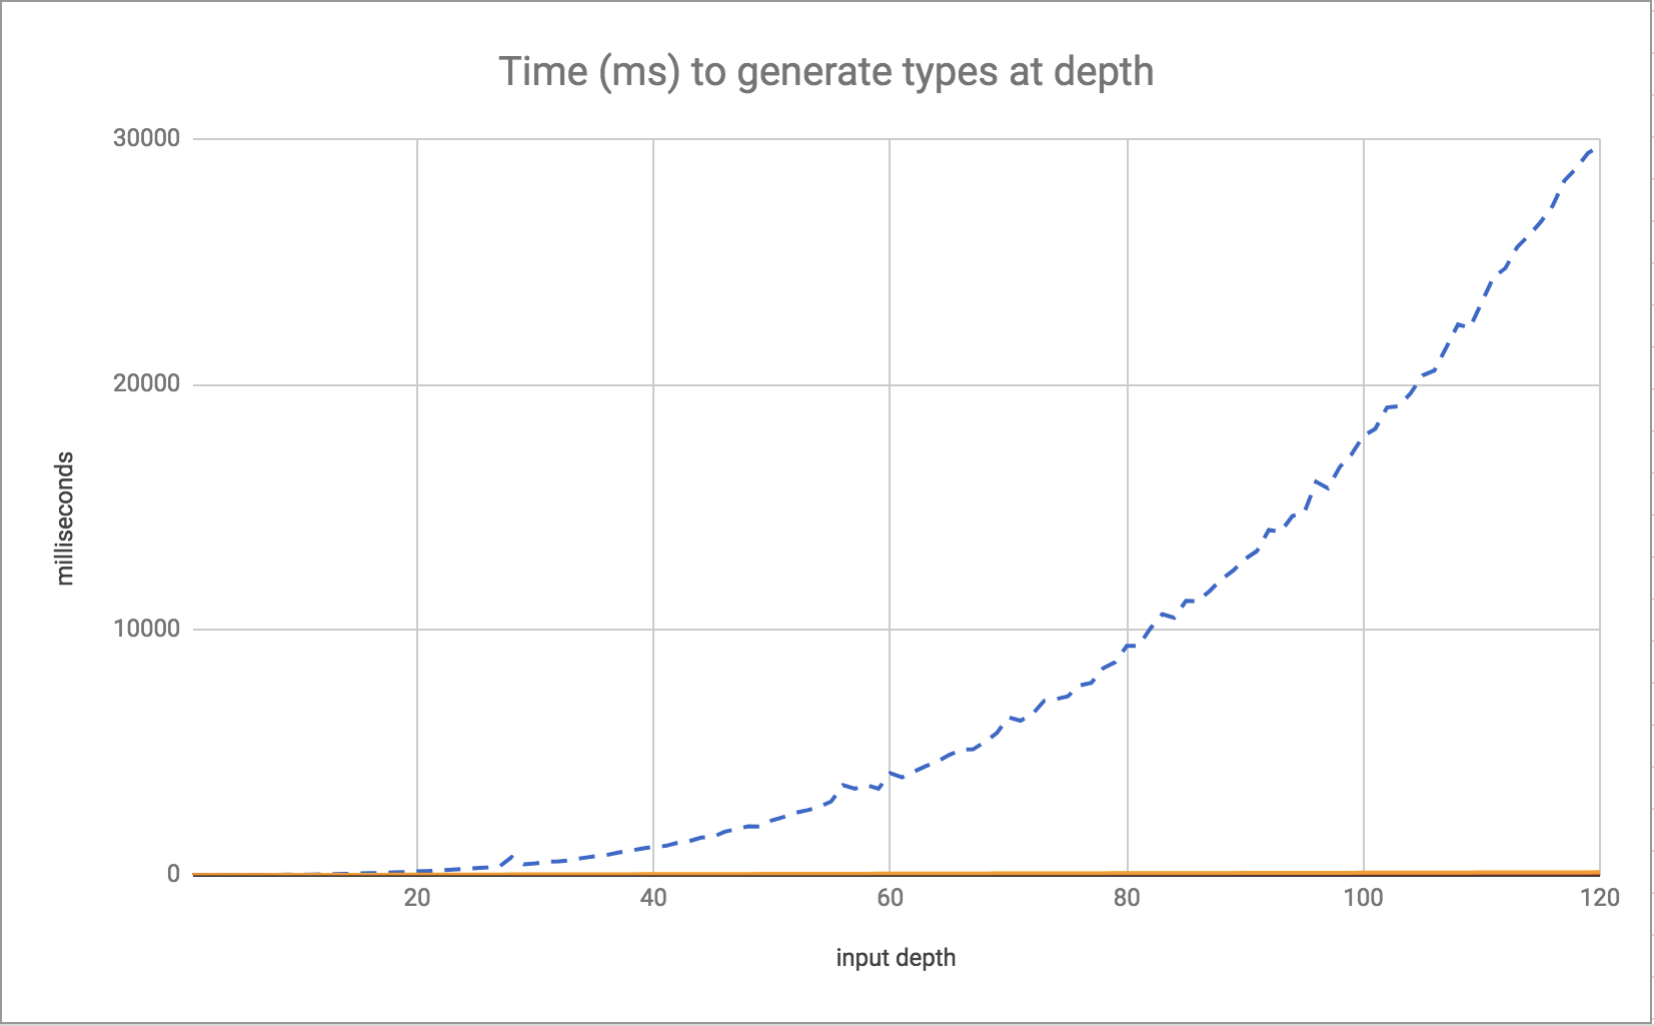
\includegraphics[width=\textwidth]{tagged-untagged-depth-bench120}

Benchmark 1 is represented by the red solid line, benchmark 2 by the
blue dotted line.

The graph shows the performance of Benchmark 1 is constant, because
the width of the largest union is always 2\ in an early phase of the reconstruction
algorithm.

The results for Benchmark 2 show the reconstruction algorithm is quadratic
with respect to the size of the largest union.

These observations are consistent with the prior theoretical analysis.

\subsection{Can space use be bounded by reducing traces as collected?}

Traces in Typed Clojure's dynamic analysis are accumulated online, and then
folded into a type environment offline. However, this fold operation is commutative
with respect to the order of traces, so performing this fold online would
eliminate the need to store traces in memory.

Space is reduced further, then, by leveraging \texttt{join} to eagerly simplify
the accumulated type environment. For example, heterogeneous maps with similar
keysets could merged, possibily using optional key entries, saving space by
preventing very large redundant unions.

It is unclear if it is possible to perform more sophisticated analyses online,
in particular the recursive type reconstruction algorithm. Since the resulting
annotations are very compressed compared to intermediate points in the analysis,
fully or partially performing this analysis online may drastically decrease space
usage where recursively defined maps are used, and very deep examples are found.

\subsection{Daikon's expressivity vs Typed Clojure's dynamic inference}

% NOTE: Not really a difference as Daikon generates structural types also.
%A significant difference between Typed Clojure's dynamic inference and Daikon's
%is that the former targets (primarily) structural types, and the latter
%nominal types. In Clojure, the primary data is in the form of data structures,
%and in Java it is in the form of classes.

Processing in Clojure is done via functions, often with immutable variables and collections.
Invariants 

The Java language requires type annotations for every variable, which Daikon utilizes.
This also means basic type information does not need to be collected about variables,
past whether they are null.

Daikon is interested in invariants between method entry and method exit. For example,
how a mutable variable might evolve over the course of a method call, or over the course
of an object's life. This kind of data is less interesting in Clojure, since mutability,
especially the usage of unsynchronized mutable local variable, is discouraged and usually
seen as for experts only.


\subsection{Space/time overhead of Daikon's dynamic tracing}

At each method entry/exit point, record the value of all variables in scope.

How to track values:

For each Java primitive, record its value.

For each Array, traverse its contents and collect hash codes
and/or primitive values.

Otherwise, get the class of the current object.

\subsection{Space/time overhead of Daikon's type inference}

\subsection{How to type check Daikon's invariants}

"Simplify" is a theorem prover for Java. Daikon can compile its invariants
to Simplify.

Simplify implements the following theories.

1. The theory of equality, \texttt{=}

2. The theory of arithmetic with functions \texttt{+}, \texttt{*}, \texttt{-},
   and relation symbols \texttt{>}, \texttt{<}, \texttt{<=}, and \texttt{>=}.

3. The theory of maps with two functions \texttt{select} and \texttt{store} (ie. get/set),
   and two additional axoims.

4. Partial orders (?)

These could be encoded in Dependent Typed Racket, since it supports propositions
in linear arithmetic constraints about variables, pairs, car, and cdr.

% Notes:
%  Java implementation:
%    Chicory does instrumentation on JVM bytecode
%     instrument_all_methods: https://github.com/codespecs/daikon/blob/master/java/daikon/chicory/Instrument.java#L409
%      add_entry_instrumentation
%     - https://github.com/codespecs/daikon/blob/master/java/daikon/chicory/Instrument.java#L825
%      add_return_instrumentation
%       - instruments return statements
%      - https://github.com/codespecs/daikon/blob/master/java/daikon/chicory/Instrument.java#L675
%     daikon.chicory.Runtime
%      - contains wrappers for values that are rewritten to?
%      - Runtime.enter(...) is called at the top of every wrapped method
%      - `dtrace_writer` records inference results
%      daikon.chicory.DaikonVariableInfo
%      - actually traverses values here
%      - arrays are traversed eagerly, but only one level
%        - subsequent levels use identityHashCode summaries


\pagebreak
\section{Question 2}

\begin{verbatim}
Examine the use of Clojure's core.spec contract system in several
real world code bases. Look at what features are used, and how precise
specifications are. Analyze how specifications address the lack of
higher-order contracts by looking at the frequency of higher-order function
contracts vs higher-order functions that omit specifications of higher-order
arguments or results.
\end{verbatim}

\subsection{What spec features are used in real systems}

\subsection{How precise are spec annotations in practice?}

\subsection{How frequently are higher-order functions annotated with higher-order specs? Why?}

\pagebreak
\section*{Question 3}

\begin{verbatim}
Write a formal model of Clojure with core.spec, and implement it in
PLT Redex. Formulate a consistency property between contracted and
uncontracted execution, and test it in redex.
\end{verbatim}

\begin{figure*}
$$
\begin{altgrammar}
  \expd{}, \e{} &::=& \x{}
                      \alt \v{} 
                      \alt {\comb {\e{}} {\e{}}} 
                      \alt {\abs {\x{}} {\t{}} {\e{}}}
                      \alt {\ifexp {\e{}} {\e{}} {\e{}}}
                      \alt {\doexp {\e{}} {\e{}}}
                &\mbox{Expressions} \\
  \v{} &::=&          \singletonmeta{}
                      \alt {\emptymap{}}
                      \alt {\num{}}
                      \alt \mapval{}
                      \alt {\closure {\openv{}} {\abs {\x{}} {\t{}} {\e{}}}}
                &\mbox{Values} \\
  \mapval{} &::=&  {\curlymapvaloverright{\v{}}{\v{}}}
                &\mbox{Map Values} \\
  \HashMapExp{}                &::=& \hmapexpressionsyntax{}
\end{altgrammar}
$$
\caption{Syntax of Terms and Specs}
\end{figure*}



\bibliography{bibliography}

\pagebreak
\appendix
\section{Experiment 1}
\label{appendix1}

This section we put our notes on the first experiment.

\begingroup
    \fontsize{5pt}{7pt}\selectfont
\begin{verbatim}
valuehash: 
- 1 fn returning fn
- 1 fn taking fn
- Note: fn takes input-stream, how to generate? are fspec generators used in `lein test`?
https://github.com/arachne-framework/valuehash/blob/fdd19b4a4c3b294d46fe7e0b50187290043b48aa/src/valuehash/specs.clj

arachne-fileset: trying to get best of both worlds (documentation but no generative testing)
- 1 fn taking pred
- Note: fn takes File
https://github.com/arachne-framework/arachne-fileset/blob/0336d2d8d273eb1e0a862641000da1bd76099626/test/user.clj#L35

dspec: utility function, checks direct HOF
- 1 fn taking pred (filter wrapper)
https://github.com/lab-79/dspec/blob/26f88e74066e381c8569d175c1bd5948a8005bd0/src/clj/lab79/dspec/util.clj

async-connect: maps of fn handlers
- 19 fspecs, for a `keys` of functions
- Note: `with-generator` suppresses all fspec generators, but that doesn't suppress
  instrumentation fn generative testing. Unsure if generative testing used.
  Takes a :netty/context, but that spec isn't defined anywhere...
https://github.com/tyano/async-connect/blob/4f30801485b68e60fc5352b8a169b6f5829d2553/src/async_connect/netty/handler.clj
- 7 fspecs, maps of fn's (channel ops)
- Note: `with-generator` suppresses generators
https://github.com/tyano/async-connect/blob/4f30801485b68e60fc5352b8a169b6f5829d2553/src/async_connect/server.clj#L46

devcards: direct HOF, also mixes ifn? checks
- 3 ifn?'s
  - 2 in map input
  - 1 fn taking fn
- 1 fspec
  - 1 fn returning fn
  - 1 fn taking map with a fn entry
- Note: alpha quality
https://github.com/olivergeorge/devcards-vs-clojure-spec/blob/385e332c21e57b097b56e899c09e99a260daf3ad/src/devcards_vs_clojure_spec/core_specs.cljc#L7

email-tool: map of fn's
- 2 fspecs
  - map args to fn
  - 1 fspec is any -> any
  - 1 fspec has easy to generate things (strings etc.)
https://github.com/andrewzhurov/email-tool/blob/fd6bf979c5534315edf0d5e2ca762a879d0c9587/src/email_tool/parts.clj#L8

bifocal: lenses, everything is HOF, sorely missing polymorphism
- 6 fspecs
  - 4 are basically any -> any
  - fn taking fn taking fn (3 nestings)
   - (s/def ::upd-f (s/fspec :args (s/cat :s any? :f fn?) :ret any?))
- 1 fn?
  - as above, mixing with fspec
https://github.com/andrewmcveigh/bifocal/blob/850e79452f4f9bc6966768055acfc7aae6671f80/src/bifocal/lens.clj#L36

triboard: fn taking fn
- 1 fspec
  - posn -> any
https://github.com/QuentinDuval/triboard/blob/dc9d60197262857bbea0756a5a395ba248929961/src/cljs/triboard/view/frame.cljs#L15

yoose: fn taking handler fn
- 1 fspec
  - 1 fn taking fn (any -> any, event handler)
https://github.com/brianium/yoose/blob/6400ed9e20f8472411c6cb0185a392cda097a0b8/src/brianium/yoose/spec.clj#L9

cljs-fn: map of fn's
- 2 fspecs (react)
  - map of fn's
  - render db/id fn
  - thunk for end of row formatting
https://github.com/briansunter/cljs-hn/blob/a15bac4535fd88d6f79a80864a0301fe3d7d8d60/src/hackernews/components/list.cljs#L15

kxix.collect: fn taking handler/processing fn's
- 2 fspecs
  - 2 fn taking fn's (handlers)
- Note: alpha, no release but not a toy
https://github.com/MastodonC/kixi.collect/blob/8a5e6a0de041f5684602235be6466afa805be92d/src/kixi/collect/aggregate.clj#L15

frereth-common: or + fn's !!!
- 5 fspecs
 - 3 fn taking fn
 - 2 fn returning fn
 - odd combination of or + fspec's
 - most (any -> any) but comments are unsure if it can be more specific
  - perhaps polymorphism might help?
- Note: unreleased, discouraged from use, but not a toy
https://github.com/jimrthy/frereth-common/blob/ff59081b170984d25e8e8192d34348ce36f7296c/src/com/frereth/common/methods.cljc#L33-L36
- 5 fspecs
  - 3 fn taking fn (bytes -> any)
  - 2 fn returning fn
https://github.com/jimrthy/frereth-common/blob/88e57bb942334124f29be1b9405bbf04c9c2af08/src/com/frereth/common/aleph.clj#L98

datomic-spec: homogeneous map with fn vals
- 1 fspec (in testing code)
  - 1 fn returning homogeneous map of fn vals (thunks that return test.check generators)
https://github.com/lab-79/datomic-spec/blob/880ab123b49da8cc79c27cd78c9a2455b260e4b9/src/cljc/lab79/datomic_spec/gen_overrides.cljc#L6

mqtt: many fspecs, contain very specific args
- 10 fspecs
 - 1 fn returning fn (connection init fn)
 - 1 fn taking fn (handler)
 - 4 fn map of fn
 - 1 fspec fn intersection (I (nil Val -> Any) (Val nil -> Any))
 - 
https://github.com/dvlopt/mqtt/blob/c7f2dcaf8d4df0a31460c16f24c5b402f21df655/src/dvlopt/mqtt/v3.clj

chu.graph: fn returning fn
- 11 fspecs
 - 14 function taking fn
 - 2 functions returns fn
 - extremely complicated dependent function specs
  - https://github.com/CharlesHD/chu.graph/blob/a820ef8456b44b1044d7f6cd9340a5504ad393de/src/chu/graph.cljc#L78-L84
  - Note: are these even used?
https://github.com/CharlesHD/chu.graph/blob/a820ef8456b44b1044d7f6cd9340a5504ad393de/src/chu/graph.cljc#L17

takelist: fn returning fn
- 1 fspec
  - 1 fn returning fn
https://github.com/alexanderkiel/takelist/blob/434ef6f6e05ca406c446b81fa5a77c7f0519c355/src/takelist/app.clj#L27

java.jdbc: seems dubious these are ever used, unless fn's are stubbed.
- 6 fspec
  - 1 fn taking fn
  - 7 fn taking map of fn
  - 1 fn returning fn
- 1 fspec commented out
  - improved custom generator needed (database ResultSet's)
https://github.com/clojure/java.jdbc/blob/64a79366fa464be75bdf4bdda133441b9d1efb26/src/main/clojure/clojure/java/jdbc/spec.clj#L124

sparkle: disjunction between map and fn
- 1 fspec (fdef return)
https://github.com/GradySimon/sparkle/blob/d5d82c37ab6be8359be7d3b5524d8b32dac452a1/src/sparkle/layer.clj#L9
 - commented out dependent :fn clause
https://github.com/GradySimon/sparkle/blob/d5d82c37ab6be8359be7d3b5524d8b32dac452a1/src/sparkle/spec.clj#L18-L24
\end{verbatim}
\endgroup

\section{Experiment 2}
\label{appendix2}

This section we put our notes on the second experiment.

\begingroup
    \fontsize{5pt}{7pt}\selectfont
\begin{verbatim}
arachne-fileset : explicitly avoids fspec, comments out more expressive specs to avoid generative behaviour
- 5 fn taking ifn?
- 2 homogeneous map of ifn?
- Comment: ;; Need to override specs here so it doesn't try to gen when I instrument
https://github.com/arachne-framework/arachne-fileset/blob/0336d2d8d273eb1e0a862641000da1bd76099626/src/arachne/fileset/specs.clj#L7

z-com : uses ifn? (probably polymorphic 1 arg function), probably doesn't make sense to gen
- 4 fn taking ifn?
- 4 heterogeneous map of ifn?
https://github.com/aw7/z-com/blob/3180acf693f620bde5c7fb9d7c300e5deb02f88a/src/z_com/standard.cljs#L18

meiro : uses ifn? (unclear how to fspec, might be possible with very specific generators)
https://github.com/defndaines/meiro/blob/19f93996b87663fec5ed70c4966d114aa4855d6b/src/meiro/backtracker.clj#L17
- 2 fn taking ifn?
- 1 fn returning ifn?
https://github.com/defndaines/meiro/blob/f4fe98f8a54ffd0cc78a671de96bcd9727904c0c/src/meiro/core.clj#L201

comfy : utility library, uses ifn? for HOF's (19 occurrences in about a dozen very polymorphic function specs)
- 16 fn taking ifn?
- 3 fn returning ifn?
	- possible transducer returns, like in (map f)
https://github.com/madstap/comfy/blob/bbca80f269a912a3a4914188d8dac29e5edaca0b/src/madstap/comfy.cljc

ferje : polymorphic "app(ly)" function uses ifn?
- 1 fn taking ifn?
	 - polymorphic
https://github.com/chourave/ferje/blob/d8a3261309a994bdbaf6e3af29fc6d22c3e51844/src/ferje/util.clj#L33

huri : 12 occurrences of ifn? (here combines `s/or` and ifn?, so fspec probably not appropriate)
- 109 fn taking ifn?
- 30 heterogeneous map ifn?
- 93 homogeneous map ifn?
https://github.com/sbelak/huri/blob/fc98c5f1870f524c1e2662980085b6a258abd5cf/src/huri/core.clj#L159-L161

arche : ifn? takes a "User Defined Type" (keyword), perhaps hard to generate?
- 6 fn taking ifn?
- 6 heterogeneous map ifn?
https://github.com/troy-west/arche/blob/1c739d178cbc5e1e1f0ac67feb64da2f8e82e099/src/troy_west/arche/spec.clj#L36

conllu-clj : ifn? for `keyfn`, but can only be one of 2 predefined def's
- 1 fn taking ifn?
https://github.com/ysmiraak/conllu-clj/blob/6bc02c8f3a28dcea871c20fb965878b21fb0c5e5/src/conllu/eval.clj#L19
- 2 fn taking ifn?
	- arbitrary transformation functions
https://github.com/ysmiraak/conllu-clj/blob/564e64a94cfde69f58dc37da183e735ebd5a07bb/src/conllu/parse.clj#L42

planck : TCP data handlers are ifn?
- 2 fn taking ifn?
https://github.com/mfikes/planck/blob/3bc8b174834cf413dbc7415f7af30955adcc27b0/planck-cljs/src/planck/socket/alpha.cljs#L11-L12

owlet : callback is ifn?
- 1 fn taking ifn?
	- callback
https://github.com/codefordenver/owlet/blob/4864e0cbc7726501cc58a1362347f07f10524ed7/src/cljs/owlet/views/confirm.cljs#L12

sqlingvo : evaluation fn is ifn? + another (latter could be enum of fns tbh)
- 2 fn returning ifn?
- 2 heterogeneous map ifn?
	- ifn's are interfaces to db
https://github.com/r0man/sqlingvo/blob/183014264e998366cdb906dbfe35a984c7d5443f/src/sqlingvo/db.cljc

proletariat : 2 HOF helpers with IFn (reduce, conj wrappers)
- 2 fn taking ifn?
	- could be polymorphic
https://github.com/LiaisonTechnologies/proletariat/blob/2a9a8cb8185785cb1d12376da21ddb97d5e43d51/src/proletariat/core.clj#L566

mazes : ifn? for predicate arg (but rest of fn is also sparsely annotated with sequential?)
- 1 fn taking ifn?
https://github.com/amacdougall/mazes/blob/1766a5fb2a3bbfc3141f44c09a2477a1ec65edef/src/cljc/mazes/generators/wilson.cljc#L36

Arcadia : listener is ifn?
- 1 fn taking ifn?
https://github.com/arcadia-unity/Arcadia/blob/a0f1ee9f3d8a5b248bb415001d2d0cb2d27527db/Source/arcadia/internal/state.clj#L52

hive : callback is ifn?
- 1 fn taking ifn?
- 1 heterogeneous map ifn?
https://github.com/hiposfer/hive/blob/f4323cc6ddba894942ba37329d4a5f7f7f974024/src/hive/services/raw/location.cljs#L12

datacore : map of callbacks is ifn? vals, + 4 function inputs as ifn?
- 14 fn taking ifn?
- 11 fn returning ifn?
- 22 heterogeneous map ifn?
- 11 homogeneous map ifn?
https://github.com/stathissideris/datacore/blob/e4ab7f4822edfccca821fb8f4f9ec81a69e9d056/src/datacore/cells.clj#L59

ambiparse : predicate is ifn?
- 1 fn returning ifn?
- 2 heterogeneous map ifn?
https://github.com/brandonbloom/ambiparse/blob/eeb047878e4990a877810ac4805a45d8cfe9acfb/src/ambiparse/gll.clj#L175
\end{verbatim}
\endgroup


\end{document}
